%=================AVANCES Y PRUEBAS=================
% SENSORES DE PULSO

\section{Módulo Gestión de Notificaciones}
Para que el usuario pueda consultar sus las notificaciones que han sido enviadas, así como configurar alguna de ellas, es necesario que siga el flujo establecido, el cual se describe a continuación.\\


\subsection{Gestión de Notificaciones}

La figura \ref{fig:GestionNotifica} se muestra el diagrama de secuencia correspondiente al login del usuario, mismo que contiene los métodos implementados en la clase JAVA, API e IU.

\begin{figure}[htbp!]
	\centering
	\fbox{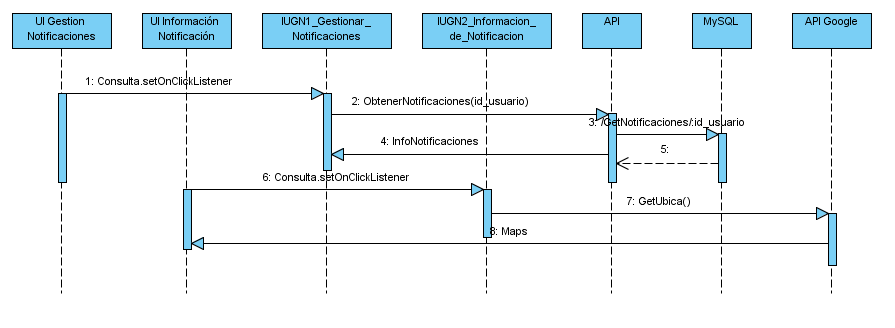
\includegraphics[width=1.0\textwidth]{AvancesPruebas/imagenes/GestionNotifica}}
	\caption{Diagrama secuencia Gestión de Notificaciones}
	\label{fig:GestionNotifica}
\end{figure}
\begin{itemize}
	\item \textbf{Login.setOnClickListener:} Es la acción que dispara el usuario, no recibe datos como parámetros, es el disparador.
	\item \textbf{isEmailValid(tx login):} Valida que el correo electrónico sea válido, se realiza la validación con base en una expresión regular.
	\item \textbf{validarPass(tx login):} Dispara una petición al API, enviando como parámetro el correo del usuario, esto para obtener el password correspondiente al correo electrónico.
	\item \textbf{/login/:tx login:} Es la ruta para la obtención del password correspondiente al correo electrónico.
\end{itemize}

\subsection{Configuración de notificaciones}

La figura \ref{fig:GestionNotifica} se muestra el diagrama de secuencia correspondiente al login del usuario, mismo que contiene los métodos implementados en la clase JAVA, API e IU.

\begin{figure}[htbp!]
	\centering
	\fbox{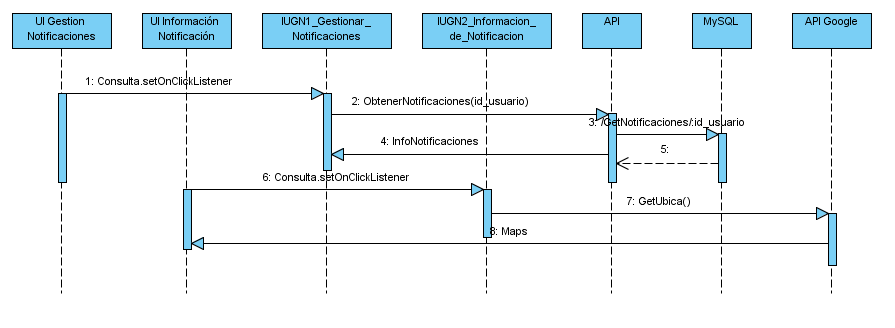
\includegraphics[width=1.0\textwidth]{AvancesPruebas/imagenes/GestionNotifica}}
	\caption{Diagrama secuencia Gestión de Notificaciones}
	\label{fig:GestionNotifica}
\end{figure}
\begin{itemize}
	\item \textbf{Login.setOnClickListener:} Es la acción que dispara el usuario, no recibe datos como parámetros, es el disparador.
	\item \textbf{isEmailValid(tx login):} Valida que el correo electrónico sea válido, se realiza la validación con base en una expresión regular.
	\item \textbf{validarPass(tx login):} Dispara una petición al API, enviando como parámetro el correo del usuario, esto para obtener el password correspondiente al correo electrónico.
	\item \textbf{/login/:tx login:} Es la ruta para la obtención del password correspondiente al correo electrónico.
\end{itemize}